\index{I-prior!model}
After selecting a RKHS/RKKS $\cF$ of functions over $\cX$ suitable for the regression problem at hand, one then proceeds to estimate the posterior distribution of the regression function.
The I-prior model \cref{eq:model1} subject to \cref{eq:model1ass} and $f\in\cF$ has the simple and convenient representation
\begin{align}\label{eq:model2}
  \begin{gathered}
    y_i = \alpha + 
    \myoverbrace{f_0(x_i) + \sum_{k=1}^n h_\eta(x_i,x_k)w_k 
    }{f(x_i)}
    + \epsilon_i \\
    (\epsilon_1,\dots,\epsilon_n)^\top \sim \N_n(\bzero, \bPsi^{-1}) \\
    (w_1,\dots,w_n)^\top \sim \N_n(\bzero,\bPsi),
  \end{gathered}
\end{align}
where $f_0:\cX\to\bbR$ is a function chosen a priori representing the ``best guess'' of $f$, and the dependence of the kernel of $\cF$ on parameters $\eta$ is emphasised through the subscript in $h_\eta:\cX\times\cX\to\bbR$.

\index{I-prior!posterior distribution}
The parameters of the I-prior model are collectively denoted by $\theta = \{\alpha,\eta,\bPsi \}$.
Given $\theta$ and a prior choice for $f_0$, the posterior regression function is determined solely by the posterior distribution of the $w_i$'s.
Using standard multivariate normal results, one finds that the posterior distribution for $\bw := (w_1,\dots,w_n)^\top$ is $\bw|\by \sim \N_n(\wtilde, \tilde\bV_w )$, where
\begin{align}\label{eq:posteriorw}
  \begin{gathered}
    \wtilde = \bPsi \bH_\eta \bV_y^{-1} (\by - \alpha\bone_n - \bff_0)
    \hspace{0.5cm}\text{and}\hspace{0.5cm}
    \tilde\bV_w = \big(\bH_\eta\bPsi\bH_\eta + \bPsi^{-1}\big)^{-1} = \bV_y^{-1},
  \end{gathered}
\end{align}
%where $\bff_0=\big(f_0(x_1),\dots,f_0(x_n) \big)^\top$, $\bH_\eta$ is the kernel matrix with $(i,j)$ entries equal to $h_\eta(x_i,x_j)$, and $\bV_y$ is the variance of the marginal distribution for $\by = (y_1,\dots,y_n)$.
using the familiar notation that we introduced in \cref{sec:introregiprior}.
For a derivation, see \cref{apx:posteriorw} \colp{\mypageref{apx:posteriorw}}.
By linearity, the posterior distribution for $f$ is also normal.

In each modelling scenario, there are a number of kernel parameters $\eta$ that need to be estimated from the data.
Assuming that the covariate space is $\cX = \cX_1\times\cdots\times\cX_p$, and there is an ANOVA like decomposition of the function space $\cF$ into its constituents spaces $\cF_1,\dots,\cF_p$, then at the very least, there are $p$ scale parameters $\lambda_1,\dots,\lambda_p$ for each of the RKHSs.
Depending on the RKHS used, there could be more kernel parameters that need to be optimised, for instance, the Hurst index for the fBm RKHS, the lengthscale for the SE RKHS, and/or the offset for the polynomial RKKS.
However, these may be treated as fixed parameters as well.
%Default settings for these parameters may be used, and if this is the case, only scale parameters need to be estimated, and the estimation procedure can be made more efficient as the kernel matrices need not be recomputed each time.
%This is explained in further detail in \hltodo{Section 4.X}.

The following subsections describe possible estimation procedures for the hyperparameters of the model.
Henceforth, for simplicity, the following additional standing assumptions are imposed on the I-prior model \cref{eq:model2}:
\begin{enumerate}[label=A\arabic*,ref=A\arabic*]
  \item \textbf{Centred responses}. Set $\alpha = 0$ and replace the responses by their centred versions $y_i \mapsto \tilde y_i = y_i - \frac{1}{n}\sum_{i=1}^n$. \label{ass:A1}  
  \item \textbf{Zero prior mean}. Assume a zero prior mean $f_0(x) = 0$ for all $x\in\cX$. \label{ass:A2} 
  \item \textbf{Iid errors}. Assume identical and independent error random variables, i.e. $\bPsi = \psi\bI_n$. \label{ass:A3} 
\end{enumerate}
Assumptions \ref{ass:A1} and \ref{ass:A2} are motivated by the discussion in \cref{sec:intercept}.
Although assumption \ref{ass:A3} is not strictly necessary, it is often a reasonable one and one that simplifies the estimation procedure greatly.

\vspace{-0.25em}
\subsection{The intercept and the prior mean}\label{sec:intercept}
\vspace{-0.25em}\index{intercept}
In most statistical models, an intercept is a necessary inclusion which aids interpretation.
In the context of the I-prior model \cref{eq:model2}, a lack of an intercept would fail to account for the correct locational shift of the regression function along the $y$-axis.
Further, when zero-mean functions are considered, the intercept serves as being the ``grand mean'' value of the responses.

The handling of an intercept to the regression model may be viewed in one of two ways.
The first is to view it as a function belonging to the RKHS of constant functions $\cF_\emptyset$, and thereby tensor summing this space to $\cF$.
The second is to simply treat the intercept as a parameter of the model to be estimated.
In the polynomial and ANOVA RKKSs, we saw that an intercept is naturally induced by the inclusion of a RKHS of constant functions in their construction.
In any of the other RKHSs described in \cref{chapter2}, an intercept would need to be added separately.
These two methods convey slightly different interpretations of the intercept: in the first method, the intercept is shrunk by an I-prior, while in the second, it is not.
Estimation is also entirely different for the two methods.

In the first method, the intercept-less RKHS/RKKS $\cF$ with kernel $h$ is made to include an intercept by modifying the kernel to be $1 + h$.
The intercept will then be implicitly taken care of without having dealt with it explicitly.
However, it can be obtained by realising that for $\alpha\in\cF_\emptyset$ the RKHS of constant functions, then $\alpha = \sum_{i=1}^n w_i$.

On the other hand, consider the intercept as a parameter $\alpha$ to be estimated.
Obtaining an estimate $\alpha$ using a likelihood-based argument is rather simple.
From \cref{eq:model2}, $\E y_i = \alpha + f_0(x_i)$ for all $i=1,\dots,n$, so the maximum likelihood (ML) estimate for $\E y$ is its sample mean $\bar y = \frac{1}{n}\sum_{i=1} y_i$, and hence the ML estimate for $\alpha$ is $\hat\alpha = \bar y - \frac{1}{n} \sum_{i=1}^n f_0(x_i)$.
Thus, assumption \ref{ass:A1} therefore implies that the ML estimate for the intercept is the sample mean of the responses.

%Finally, the estimation of $\alpha$ under a fully Bayesian treatment is possible by assuming an appropriate hyperprior on it, such as a conjugate normal prior $\N(a,A^{-1})$.
%If so, the conditional posterior of $\alpha$ given $\bw$, $\eta$, $\bPsi$ and $f_0$ is also normal with mean $\tilde a$ and variance $\tilde A$, where
%\[
%  \tilde A = \sum_{i,j=1}^n \psi_{ij} + A
%  \hspace{0.5cm}\text{and}\hspace{0.5cm}
%  \tilde a = \tilde A^{-1}\left( \sum_{i=1}^n [(\by-\bff_0-\bH_\eta \bw)\bPsi]_i + Aa \right).
%\]
%This fact can be used, say, in conjunction with a Gibbs sampling procedure treating the rest of the unknowns as random.
%Note that the posterior mean for $\alpha$ is
%\begin{align*}
%  \E [\alpha|\by] 
%  &= \E_\bw\big[ \E [\alpha|\by,\bw] \big] 
%  = \frac{\sum_{i,j=1}^n \psi_{ij}(y_i-f_0(x_i)) + Aa}{\sum_{i,j=1}^n \psi_{ij} + A},
%\end{align*}
%which, in the iid errors case, is seen to be a weighted sum of the ML estimate $\hat\alpha$ and the prior mean $a$.
%Unless there is a strong reason to add prior information to the intercept, the ML estimate seems to be the simplest approach.
%Assumption \ref{ass:A1} therefore implies a ML estimation of the intercept parameter.

\subsection{Direct optimisation}

\index{I-prior!log-likelihood}
\index{maximum likelihood!estimate}
\index{quasi-Newton method}
\index{quasi-Newton method|seealso{Newton method}}
Under assumptions \ref{ass:A1}--\ref{ass:A3}, a direct optimisation of the parameters $\theta=\{\eta,\bPsi=\psi\bI_n \}$ using the log-likelihood of $\theta$ is straightforward to implement.
Denote $\bSigma_\theta := \psi\bH_\eta^2 + \psi^{-1}\bI_n = \bV_y$.
From \cref{eq:model2}, the marginal log-likelihood of $\theta$ is given by
\begin{align}
  L(\theta)
  &= \log \int p(\by|\bw,\theta)p(\bw|\theta) \dint \bw \nonumber \\
  &= -\half[n]\log 2\pi - \half\log\vert \bSigma_\theta \vert - \half \tilde\by^\top \bSigma_\theta^{-1} \tilde\by \label{eq:marglogliky},
\end{align}
which is the log-likelihood of a zero mean multivariate normal distribution with covariance matrix $\bSigma_\theta$.
This closed-form expression of the integral \cref{eq:marglogliky} stems from the fact that the (conditional) likelihood and the I-prior are both Gaussian.
Note that the term `marginal' refers to the fact that we are averaging out the random function represented by $\bw$.

\index{Cholesky decomposition}
For Gaussian process regression (GPR), direct optimisation is typically done using the conjugate gradients method in conjunction with a Cholesky decomposition on the covariance kernel to maintain stability \citep{rasmussen2006gaussian}. 
We opt for a quasi-Newton algorithm (L-BFGS algorithm, \cite{nocedal2006numerical}) \index{L-BFGS algorithm} with an eigendecomposition of the kernel matrix $\bH_{\eta} = \bV \, \text{diag}(u_1,\dots,u_n) \, \bV^\top$ instead.
This procedure is relatively robust to numerical instabilities and is better at ensuring positive definiteness of the covariance kernel.
%The eigendecomposition is performed using the \pkg{Eigen} \proglang{C++} template library and linked to \pkg{iprior} using \pkg{Rcpp} \citep{eddelbuettel2011rcpp}.
%The hyperparameters are transformed by the \pkg{iprior} package so that an unrestricted optimisation using the quasi-Newton L-BFGS algorithm provided by \code{optim()} in \proglang R.
%Note that minimisation is done on the deviance scale, i.e. minus twice the log-likelihood.
Since $\bH_{\eta}$ is a symmetric matrix, we have that $\bV\bV^\top = \bI_n$, and thus
\begingroup
\setlength{\abovedisplayskip}{6pt}
\setlength{\belowdisplayskip}{8pt}
\begin{align*}
  \bV_y 
  &= \psi\bV \, \text{diag}(u_1^2,\dots,u_n^2) \, \bV^\top + \psi^{-1} \bV\bV^\top \\
  &= \bV \, \text{diag} (\psi u_1^2 + \psi^{-1},\dots,\psi u_n^2 + \psi^{-1}) \, \bV^\top 
\end{align*}
\endgroup
for which the inverse and log-determinant is easily obtainable.
To be explicit, the log-likelihood is given by
\begingroup
\setlength{\abovedisplayskip}{8pt}
\setlength{\belowdisplayskip}{6pt}
  \begin{align}
    \begin{split}
      L(\theta) 
      ={}& -\half[n]\log 2\pi - \half\sum_{i=1}^n\log(\psi u_i^2 + \psi^{-1}) \\
      &- \half \tilde\by^\top \bV \, \text{diag} \left(\frac{1}{\psi u_1^2 + \psi^{-1}},\dots,\frac{1}{\psi u_n^2 + \psi^{-1}}\right) \, \bV^\top \tilde\by
    \end{split}
  \end{align}
\endgroup

The direct optimisation method can be prone to local optima, in which case repeating the optimisation at different starting points and choosing the one which yields the highest likelihood is one way around this.
On a practical note, parameters are best transformed so that optimisation of these parameters are done on an unrestricted scale (e.g. $\log \psi$).

\begin{figure}[hbt]
  \centering
  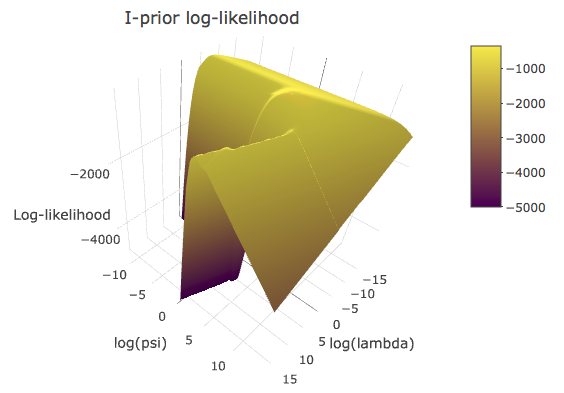
\includegraphics[width=0.75\textwidth]{figure/04-iprior-ridge-2}
  \caption[A typical log-likelihood surface plot of I-prior models.]{A typical log-likelihood surface plot of I-prior models, in which there are two ridges. The maximum occurs along one of the two ridges, or sometimes at the intersection. Clearly, different initialisations can lead optimisation algorithms to either ridge and possibly converge to a local optima.}
  \label{fig:ipriorridge}
\end{figure}

\index{Fisher information!Gaussian}
\index{standard error}
Let $\bU$ be the Fisher information matrix for $\theta \!\in\!\bbR^q$.
Standard calculations \colp{\cref{apx:fishermultinormal}, \mypageref{apx:fishermultinormal}} show that under the marginal distribution $\tilde\by \sim \N_n\big(\bzero, \bSigma_\theta \big)$, the $(i,j)$'th coordinate of $\bU$ is 
\begin{equation}
  u_{ij} = 
  \half \tr\left(
  \bSigma_\theta^{-1} \frac{\partial\bSigma_\theta}{\partial\theta_i}
  \bSigma_\theta^{-1} \frac{\partial\bSigma_\theta}{\partial\theta_j} 
  \right), \hspace{0.5cm}i,j=1,\dots,q,
\end{equation}
where the derivative of a matrix with respect to a scalar is the element-wise derivative of the matrix.
With $\hat\theta$ denoting the ML estimate for $\theta$, under suitable conditions, $\surd n (\hat\theta - \theta)$ has an asymptotic multivariate normal distribution with mean zero and covariance matrix $\bU^{-1}$ \citep{casella2002statistical}.
In particular, the standard error for $\theta_k$ is the $k$'th diagonal element of $\bU^{-1/2}$.

\subsection{Expectation-maximisation algorithm}
\label{sec:emiprior}

\index{EM algorithm}
Evidently, the model in \cref{eq:model2} resembles a random-effects model, for which the EM algorithm is easily employed to estimate its hyperparameters.
Assume \ref{ass:A1}--\ref{ass:A3} holds.
By treating the complete data as $\{\by,\bw \}$ and the $w_i$'s as ``missing'', the $t$'th iteration of the E-step entails computing
\begin{align}
  Q(\theta) 
  &= \E_\bw \left( \log p(\by, \bw | \theta) \big\vert\, \by,\theta^{(t)} \right) \nonumber \\
  &= \E_\bw \left( \const 
  + \cancel{\half[n]\log\psi}
  - \half[\psi] \Vert \tilde\by - \bH_\eta\bw \Vert^2  
  - \cancel{\half[n]\log\psi}
  - \half[\psi^{-1}] \Vert \bw \Vert^2
  \,\Big\vert\, \by,\theta^{(t)} \right) \label{eq:QfnEstep} \\
  &=  \const - \half[\psi] \tilde \by^\top \tilde \by
  - \half \tr \Big( (
  \myoverbrace{\psi\bH_\eta^2 + \psi^{-1}\bI_n}{\bSigma_\theta} 
  )\tilde\bW^{(t)} \Big)
  + \psi\tilde\by^\top\bH_\eta\wtilde^{(t)}, \nonumber
\end{align}
where $\tilde\bw^{(t)} = \E \big( \bw|\by,\theta^{(t)} \big)$ and $\tilde\bW^{(t)} = \E\big( \bw\bw^\top|\by,\theta^{(t)} \big)$ are the first and second posterior moments of $\bw$ calculated at the $t$th EM iteration.
These can be computed directly from \cref{eq:posteriorw}, substituting for $\theta^{(t)} = \{\eta^{(t)}, \psi^{(t)} \}$ as appropriate.

The M-step assigns $\theta^{(t+1)}$ the value of $\theta$ which maximises the $Q$ function above.
This boils down to solving the first order conditions
\begin{align}
  \frac{\partial Q}{\partial\eta}
  &= -\half \tr \left(\frac{\partial \bSigma_\theta}{\partial\eta} \tilde\bW^{(t)} \right) + \psi  \cdot \tilde\by ^\top \frac{\partial \bH_\eta}{\partial\eta} \tilde\bw^{(t)} \label{eq:emtheta} \\
  \frac{\partial Q}{\partial\psi}
  &= -\half \tilde\by^\top\tilde\by - \tr \left(\frac{\partial \bSigma_\theta}{\partial\psi} \tilde\bW^{(t)} \right) + \tilde\by^\top \bH_\eta \tilde\bw^{(t)} \label{eq:empsi}
\end{align}
equated to zero.
As $\partial\bSigma_\theta/\partial\psi = \bH_\eta^2 - \psi^{-2}\bI_n$, the solution to \cref{eq:empsi} for $\psi$ admits a closed form given values for $\eta$:
\begin{align}\label{eq:closedformpsi}
  \psi^{(t+1)} = 
  \left\{ \frac{\tr \Wtilde^{(t)}}{\tilde\by^\top\tilde\by + \tr(\bH_\eta^2\Wtilde^{(t)}) - 2\tilde\by^\top\bH_\eta\wtilde^{(t)}} \right\}^{1/2}.
\end{align}
We use this fact to form a sequential updating scheme $\eta^{(t)} \to \psi^{(t+1)} \to \eta^{(t+1)} \to \cdots$, and this form of the EM algorithm is known as the \emph{expectation conditional maximisation} algorithm \citep{meng1993maximum}.\index{ECM algorithm}
\index{ECM algorithm}
Now, the solution to \cref{eq:emtheta} can also be found in closed-form given values $\psi$, for many models, but in general, this is not the case. 
In cases where closed-form solutions do exist for $\eta$, then it is just a matter of iterating the update equations until a suitable convergence criterion is met (e.g. no more sizeable increase in successive log-likelihood values).
In cases where closed-form solutions do not exist for $\eta$, the $Q$ function is again optimised with respect to $\eta$ using the gradient-based algorithms.

\index{numerical issues}
In our experience, the EM algorithm is more stable than direct maximisation, in the sense that the EM steps increase the likelihood in a gentle manner that prevents sudden explosions of the likelihood.
In contrast, the search direction using gradient-based methods can grow the likelihood too quickly and potentially causes numerical errors to creep in.
%The reason for this is that the $Q$ function is generally convex in the parameters (at the very least, it is convex in each coordinate of $\theta$, in most cases anyway).
As such, the EM is especially suitable if there are many scale parameters to estimate, but on the flip side, it is typically slow to converge.
The \pkg{iprior} package provides a method to automatically switch to the direct optimisation method after running several EM iterations.
This then combines the stability of the EM with the speed of direct optimisation.
%Section X also describes various strategies to run the EM algorithm efficiently.

%As a final remark, it is well known that the EM algorithm increases the value of the log-likelihood at each iteration.
%It is also known that the EM sequence $\theta^{(t)}$ eventually convergences to some $\theta^*$, but the fact that $\theta^*$ is the ML estimate is not guaranteed.
%The paper by \citet{wu1983convergence} details the conditions necessary for the EM to produce ML estimates.
%If the EM tends to get stuck in some local maxima of the likelihood, then a general strategy is to restart the EM from multiple starting values. 


\subsection{Markov chain Monte Carlo methods}

\index{MCMC}
\index{HMC}
For completeness, it should be mentioned that a full Bayesian treatment of the model is possible, with additional priors on the set of hyperparameters.
Markov chain Monte Carlo (MCMC) methods can then be employed to sample from the posteriors of the hyperparameters, with point estimates obtained using the posterior mean or mode, for instance.
Additionally, the posterior distribution encapsulates the uncertainty about the parameter, for which inference can be made.
Posterior sampling can be done using Gibbs-based methods in \pkg{WinBUGS} \citep{lunn2000winbugs} or \pkg{JAGS} \citep{plummer2003jags}, and both have interfaces to \proglang{R} via \pkg{R2WinBUGS} \citep{sturtz2005r2winbugs} and \pkg{runjags} \citep{denwood2016runjags} respectively.
Hamiltonian Monte Carlo (HMC) sampling is also a possibility, and the \proglang{Stan} project \citep{carpenter2016stan} together with the package \pkg{rstan} \citep{rstan}  makes this possible in \proglang{R}.

On the software side, all of these MCMC packages require the user to code the model individually, and we are not aware of the existence of MCMC-based packages which are able to estimate GPR models.
This makes it inconvenient for GPR and I-prior models, because in addition to the model itself, the kernel functions need to be coded as well and ensuring computational efficiency would be a difficult task.
%Note that this full Bayesian method is not implemented in \pkg{iprior}, but described here for completeness.

Speaking of efficiency, it is more advantageous to marginalise the I-prior and work with the marginal model \cref{eq:marglogliky}, rather than the hierarchical specification \cref{eq:model2}.
The reason for this is that the latter model has a parameter space whose dimension is $O(n)$, while the former only samples the hyperparameters.
Note that the marginal model \cref{eq:marglogliky} cannot then be sampled efficiently using a Gibbs procedure as the Gibbs conditionals are not of closed-form.
Instead, Hamiltonian MC should be used, which does not depend on model conjugacy.
%The posterior sampling for the $w_i$'s in (equivalently, the posterior Gaussian process $f(x) = \sum_{i=1}^n h_\lambda(x,x_i)w_i$) is performed using the normal posterior distribution in \cref{eq:posteriorw}.

\subsection{Comparison of estimation methods}
\label{sec:compareestimation}

\index{smoothing model}
Consider a one-dimensional smoothing example, for which $n=150$ data pairs $(y_i,x_i)$ have been generated according to the relationship 
\begin{align}\label{eq:examplesmoothingdata}
  \begin{gathered}
    y_i = \const + \myoverbrace{
    0.35 \, \phi(x_i|1,0.8^2) + 0.65 \, \phi(x_i|4,1.5^2)
    + \ind(x_i > 4.5)\, e^{1.25(x_i-4.5)}\phantom{\Big)}
    }{f_\text{true}(x_i)} + \epsilon_i,
  \end{gathered}
\end{align}
where $\phi(\cdot|\mu,\sigma^2)$ is the probability density function of a normal distribution with mean $\mu$ and variance $\sigma^2$.
The observed $y_i$'s are thought to be noisy versions of the true points, in which $\epsilon_i$ follows an indescript, not necessarily normal, distribution.
The predictors $x_1,\dots,x_n$ have been sampled roughly from the interval $(-1,6)$, and the sampling was intentionally not uniform so that there is slight sparsity in the middle.
\cref{fig:examplesmoothingdata} plots the sampled points and the true regression function.

\begin{figure}[hbt]
  \centering
  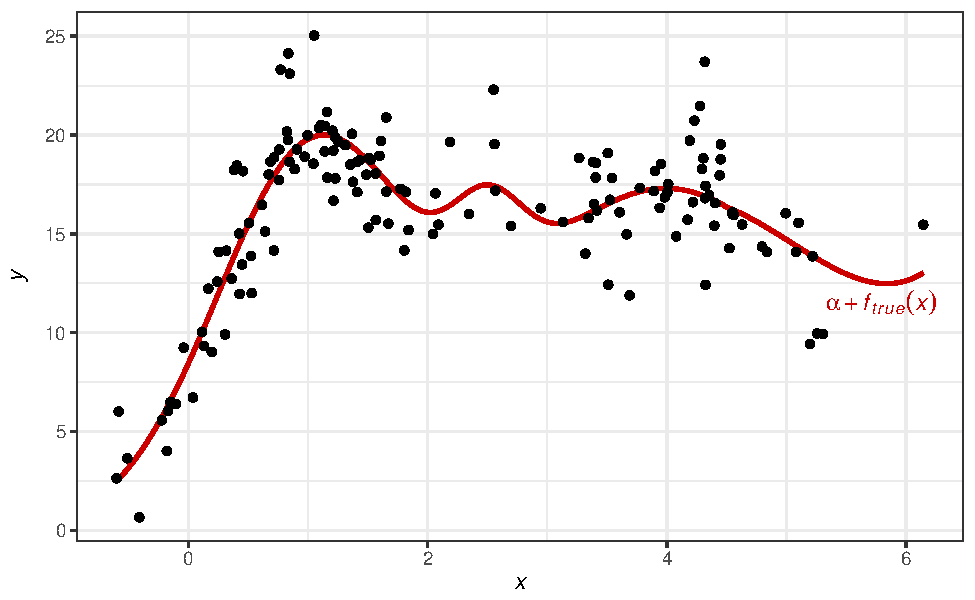
\includegraphics[width=0.8\textwidth]{figure/04-example_data}
  \caption[A plot of the toy data set for regression]{A plot of the sampled data points according to  \cref{eq:examplesmoothingdata}, with the true regression function superimposed.}
  \label{fig:examplesmoothingdata}
\end{figure}

\index{fBm kernel/RKHS}
\index{distribution!folded-normal}
We attempt to estimate $f_\text{true}$ by a function $f$ belonging to the fBm-0.5 RKHS $\cF_\lambda$, with an I-prior on $f$.
There are two parameters that need to be estimated: the scale parameter $\lambda$ for the fBm-0.5 RKHS, and the error precision $\psi$.
These can be estimated using the maximum likelihood methods described above, namely by direct optimisation using a quasi-Newton algorithm, and the EM algorithm.
These two methods are implemented in the \pkg{iprior} package. 
A full Bayesian treatment is possible, and we use the \pkg{rstan} implementation of \proglang{Stan} to perform Hamiltonian Monte Carlo sampling of the posterior densities.
A vague prior choice for $\lambda$ and $\psi$ are prescribed, namely
\[
  \lambda,\psi \iid \N_+(0,100),
\]
where $\N_+(0,\sigma^2)$ represents the \emph{folded-normal} distribution\footnote{The random variable $X \sim \N_+(\mu,\sigma^2)$ has the density $p(x) = \phi(x|\mu,\sigma^2)\ind(x \geq 0)$.}\footnote{Note that a single scale parameter $\lambda$ is not identified in sign, and is thus constrained to the positive reals. This is applicable in both likelihood-based and Bayesian methods.\index{identifiability}}.
We have also set an improper prior density $p(\alpha) \propto \const$ for the intercept.
The advantage of HMC is that efficiency is not dictated by conjugacy, so there is freedom to choose any appropriate prior choice on the parameters.

\begin{table}[hbt]
\centering
\caption{Table comparing the estimated parameter values, (marginal) log-likelihood values, and also time taken for the three estimation methods.}
\label{tab:comparemethodsestimate}
\begin{tabular}{@{}lrrr@{}}
\toprule
               & Direct optimisation & EM algorithm & Hamiltonian MC          \\ \midrule
Intercept ($\alpha$)      & 16.1 (0.35)           & 16.1 (0.35)    & 16.1 (0.17)  \\
Scale ($\lambda$)      & 5.01 (1.23)         & 5.01 (1.26)  & 5.61 (1.42)     \\
Precision ($\psi$)         & 0.236 (0.03)        & 0.236 (0.03) & 0.237 (0.03)\\[0.5em]
Log-density    & -339.7              & -339.7       & -341.1                  \\
Predictive RMSE & 0.574               & 0.575        & 0.582                   \\[0.5em]
Iterations     & 12                  & 266          & 2000                    \\
Time taken (s) & 0.96                & 3.65         & 232                     \\ \bottomrule
\end{tabular}
\end{table}

\cref{tab:comparemethodsestimate} tabulates the estimated parameter values, (marginal) log-likelihood values, and also time taken for the three estimation methods.
The three methods concur on the estimated parameter values, although the scale parameter has been estimated slightly differently, which is possibly attributed to the effect of the prior for $\lambda$.
The resulting log-likelihood value for the Bayesian method is lower than the ML methods, which also took the longest to compute.
Although the EM algorithm took longer than the direct optimisation method to compute, the time taken per iteration is significantly shorter than one Newton iteration.
%In this simple example, there were no numerical issues encountered with the direct optimisation method, but in more complex examples (see \hltodo{Section X}), instabilities could arise.
